\definecolor{blued}{RGB}{0,122,255}
\definecolor{redd}{RGB}{255,59,48}
\definecolor{cyand}{RGB}{50,173,230}
\definecolor{greend}{RGB}{52,199,89}
\subsection{Übersicht}
Die Spielwelt basiert auf einem Terrain mit quadratischer Grundfläche. Mit Space Partitioning Algorithmen werden innerhalb des Terrains Levels erstellt. Diese werden durch Korridoren miteinander verbunden, sodass eine zusammenhängende Spielwelt entsteht. Zu dem Terrain werden Masken erstellt, die Levels, Korridore und weitere Objekte und Bereiche markieren. Mithilfe der Masken und Bildfiltern, sowie Perlin-Noise werden Bereiche des Terrains modifiziert, um eine nicht planare Spielwelt zu erhalten. Innerhalb der Levels wird durch L-Systeme generierte Vegetation an zufälligen Postitionen in der Welt platziert. Dabei wird ein Mindestabstand zwischen platzierten Objekten eingehalten, so dass innerhalb der Levels alle Bereiche für den Spieler erreichbar bleiben. Weiterhin erhält das Terrain anhand der Masken Texturen. Zu dem fertigen Terrain mit platzierten Objekten wird ein NavMesh erstellt. Da alle Objekte mit einem dem AgentRadius des NavMesh angepassten Mindestabstand platziert werden, entsteht ein zusammenhängendes Navmesh. 


\subsection{Generierung von Levels mit Space Partitioning}
Zunächst wird die Seitenlänge der quadratischen Spielwelt festgelegt. Mithilfe von Space Partitioning Algorithmen wird die Spielwelt in Bereiche unterteilt, in denen Levels platziert werden können. Dabei kann die Partitionierung mit $2$-d-Bäumen oder Quadtrees erfolgen. Die Ausgangsfläche wird so lange unterteilt, bis eine weitere Unterteilung eine Mindestgröße unterscheidet. Die Ausgabe des Algorithmus besteht aus Rechtecken, in denen kleinere, rechteckige Levels platziert werden. Dabei kann über Parameter für alle vier Seiten der Abstand zu den Begrenzungen des Rechtecks durch ein Intervall aus Minimum und Maximum angegeben werden. Die Abstände werden in den jeweiligen Intervallen zufällig gewählt. So sind die Level durch Zwischenräume voneinander getrennt. Die Größe der Spielwelt, sowie die Parameter zur Begrenzung der Größe und Platzierung der Levels sind ganzzahlig. Damit lässt sich die Spielwelt in Einheitsquadrate mit jeweils einem Quadratmeter Flächeninhalt einteilen, was die Platzierung von Objekten in Levels, das Setzen von freien Pfaden, sowie die Generierung des Terrains vereinfacht.


\subsection{Levels}
Levels in der Spielwelt haben eine rechteckige Grundfläche und enthalten Spawnpunkte für Kreaturen, Vegetation und freie Pfade, die ein Durchqueren der Level unabhängig von den zufällig platzierten Objekten ermöglichen.
Zu jedem Level wird ein zweidimensionales Array \texttt{free} mit Einträgen vom Typ \texttt{bool} gespeichert. Das Array hat die Dimensionen der Grundfläche des Levels, sodass zu jeder ganzzahligen, zum Level relativen Koordinate auf der Grundfläche des Levels ein Eintrag im Array existiert. Ist der Eintrag im Array für eine Koordinate \texttt{true}, so ist das Einheitsquadrat an dieser Koordinate in der Spielwelt frei, andernfalls befindet sich hier ein platziertes Objekt oder es soll an dieser Position kein weiteres Objekt platziert werden.
 
\subsubsection{Freie Pfade in Levels}
Da die Levels rechteckige Grundfläche haben, hat jedes Level eine linke, rechte, vordere und hintere Seite. Zu jedem Level werden Punkte auf der Grundfläche gespeichert, an denen anliegende Korridore beginnen oder enden. Die Punkte befinden sich auf einer der vier Seiten des Levels. Damit keine Bereiche der Spielwelt durch platzierte Objekte abgeschnitten werden, muss von jedem anliegenden Korridor jeder andere anliegende Korridor durch einen durch das Level führenden Pfad erreichbar sein. Die Pfade  werden vor der Platzierung von Objekten definiert. Dazu werden alle Paare von Punkten anliegender Korridoren aufgezählt und mit einem naiven Algorithmus wird ein Pfad gefunden, der die Punkte jedes Paares miteinander verbindet. Die Lage der beiden Punkte auf den Seiten des Levels kann durch drei Fälle unterschieden werden. Im ersten Fall liegen beide Punkte auf der gleichen Seite. Da dieser Fall nach dem oben beschriebenen Verfahren zur Verbindung von Levels über die von einem Space Partitioning Algorithmus berechnete Baumstruktur nicht eintritt, sondern jede Seite des Levels maximal einen anliegenden Korridor haben kann, wird er nicht behandelt. Falls die Punkte auf gegenüberliegenden Seiten liegen, wird ein Pfad aus drei geraden Segmenten gebildet. Dazu wird ein zufälliger Punkt zwischen den Seiten gewählt auf dem das mittlere, zu beiden Seiten parallele Segment des Pfades liegt. Das mittlere Segment wird über gerade Segmente mit den beiden an den Seiten liegenden Punkten verbunden. Im letzten Fall liegen die Punkte auf miteinander verbunden Seiten, wie z.B. auf der hinteren und linken Seite und können durch einen eindeutigen Pfad, der aus zwei geraden Segmenten besteht verbunden werden. Die letzten beiden Fälle sind in Abbildung \ref{fig:wg_levelconnect} dargestellt. Die Breite der Pfade ist durch einen minimalen und einen maximalen Wert begrenzt und wird zufällig gewählt. Einheitsquadrate im Level, durch die Pfade verlaufen werden durch einen \texttt{false}-Eintrag im \texttt{free} Array des Levels als belegt markiert.
\begin{figure}
\centering\hfill
    \begin{subfigure}[b]{0.4\textwidth}
    \centering
        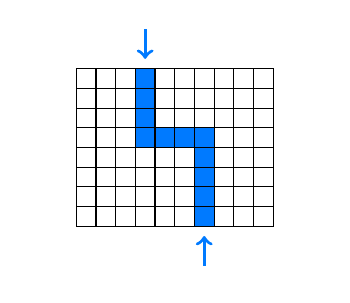
\begin{tikzpicture}
            \node at (-0.5,0){};
            \node at (3,-2.5,0){};
            \draw[fill = blued] (0.75,0) rectangle++(0.25,-1) rectangle++(0.75,0.25) rectangle++(-0.25,-1.25);
            \draw[very thick, blued, ->] (0.875,0.5) to ++(0,-0.375);
            \draw[very thick, blued, ->] (1.625,-2.5) to ++(0,0.375);
            \foreach \x in {0,...,9}
                \foreach \y in {0,...,7} 
                    {\draw ({\x*0.25},{\y*-0.25}) rectangle++(0.25,-0.25);}
        \end{tikzpicture}
        \subcaption{Fall 1}
        \label{fig:wg_levelconnect_sub1}
    \end{subfigure}\hspace*{2bp}
    \begin{subfigure}[b]{0.4\textwidth}
    \centering
        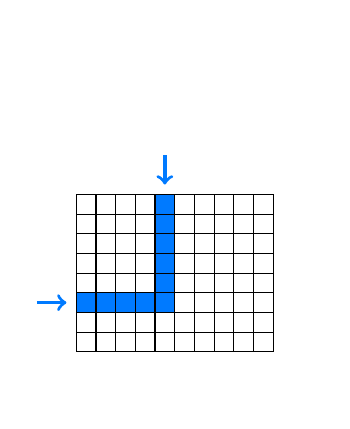
\begin{tikzpicture}
            \node at (-0.5,2){};
            \node at (3,-2.5,0){};
            \draw[fill = blued] (1,0) rectangle++(0.25,-1.5) rectangle++(-1.25,0.25);
            \draw[very thick, blued, ->] (1.125,0.5) to ++(0,-0.375);
            \draw[very thick, blued, ->] (-0.5,-1.375) to ++(0.375,0);
            \foreach \x in {0,...,9}
                \foreach \y in {0,...,7} 
                    {\draw ({\x*0.25},{\y*-0.25}) rectangle++(0.25,-0.25);}
        \end{tikzpicture}
        \subcaption{Fall 2}
        \label{fig:wg_levelconnect_sub2}
    \end{subfigure}
    \hfill
    \caption[Verbinden von anliegenden Korridoren in Levels.]{Verbinden von anliegenden Korridoren in Levels. \ref{fig:wg_levelconnect_sub1}: Punkte befinden sich auf gegenüberliegenden Seiten des Levels. \ref{fig:wg_levelconnect_sub2}: Punkte liegen auf benachbarten Seiten des Levels. Der generierte Pfad ist blau markiert.}
    \label{fig:wg_levelconnect}
\end{figure}

\subsubsection{Platzierung von Objekten und Spawnpunkten}
Objekte, wie zum Beispiel Pflanzen werden an zufällig gewählten Positionen im Level platziert. Dazu wird das zu jedem Level gespeicherte \texttt{free} Array genutzt. Zu einem Objekt das platziert werden soll muss die Breite $w$ und Höhe $h$ der Fläche, die das Objekt benötigt vorher bekannt sein. Dabei wird gefordert, dass beide Werte ungerade ganze Zahlen sind. Es wird angenommen, dass sich das Objekt zentriert innerhalb dieser Fläche befindet, wobei sich das tatsächliche Objekt nicht notwendigerweise bis zu den durch $w$ und $h$ gegebenen Begrenzungen ausdehnen muss. Bei der Platzierung des Objektes müssen vorher platzierte Objekte und sich im Level befindende freie Pfade berücksichtigt werden. Es wird eine Position im Level gesucht, an der das Objekt mittig platziert werden kann und dabei nicht mit anderen Objekten oder freien Pfaden kollidiert. Falls $w=h=1$ ist, kann eine beliebige Position im Level gewählt werden, an der $\texttt{free}$ den Eintrag $\texttt{true}$ enthält. Andernfalls wird ein zusätzliches Array $\texttt{a}$ mit den gleichen Dimensionen wie $\texttt{free}$ vom Typ $\texttt{float}$ verwendet. Zunächst wird das Array \texttt{free} in das Array \texttt{a} mit der Zuordnung $\texttt{false}\mapsto 1.0, \texttt{true}\mapsto 0.0$ abgebildet. Das Array \texttt{a} wird nun so modifiziert, dass an Positionen mit dem Wert $0.0$ das Objekt kollisionsfrei platziert werden kann. Um Kollisionen mit anderen Objekten oder Pfaden zu verhindern, werden zwei Faltungsfilter verwendet. Es wird eine Matrix $F_w$ für die horizontale und eine Matrix $F_h$ für die vertikale Ausdehnung des Objektes wie folgt definiert. \begin{align*}
    F_w = \begin{bmatrix}
        1&1&1
    \end{bmatrix} && F_h = \begin{bmatrix}
        1\\1\\1
    \end{bmatrix}
\end{align*}
Mithilfe der Faltungsfilter werden Bereiche um bereits platzierte Objekte erkannt, an denen die Platzierung eines neuen Objektes zu einer Kollision führen würde. Angenommen das Level, in dem das Objekt platziert werden soll, hat die Breite $L_w$ und Höhe $L_h$. Falls $w\ge 3$ ist, wird zunächst $\texttt{a}$ mit $F_w$ gefaltet, d.h. für alle $i,j$ mit $1 \le i \le L_w-2, 0\le j\le L_H - 1$ wird \[\texttt{a}[i,j] = a[i-1,j] +  a[i,j] + a[i+1,j]\] gesetzt. Anschließend werden die Einträge in \texttt{a}, die unmittelbar an der linken und rechten Seite des Levels anliegen auf $1.0$ gesetzt, um eine Ausdehnung des Objektes über die Begrenzungen des Levels zu verhindern. Analog wird, falls $h\ge 3$ ist, $\texttt{a}$ mit $F_h$ gefaltet, d.h. für $0\le i\le L_w-1$ und $1\le j\le L_h-2$ wird \[\texttt{a}[i,j] = \texttt{a}[i,j-1] + \texttt{a}[i,j] + \texttt{a}[i,j+1]\] gesetzt. Die Einträge unmittelbar an der vorderen und hinteren Seite des Levels werden auf $1.0$ gesetzt. Zuletzt wird die Faltungsoperation mit $F_w$ $\lfloor w/2\rfloor-1$-mal wiederholt und die Faltungsoperation mit $F_h$ wird $\lfloor h/2\rfloor-1$-mal wiederholt. Bei den Wiederholungen müssen keine Einträge nahe der Seiten des Levels gesetzt werden, da die in der ersten Iteration der Operationen mit $F_w$ und $F_h$ gesetzten Einträge durch die Wiederholungen erweitert werden. An allen Positionen im Level, an denen das Array  \texttt{a} den Wert $0.0$ enthält, kann das Objekt kollisionsfrei platziert werden. Eine solche Position wird zufällig ausgewählt und in $\texttt{free}$ auf $\texttt{false}$ gesetzt. Zusätzlich wird die umliegende, durch $w$ und $h$ beschränkte Fläche, die das Objekt in der Welt einnimmt auf $\texttt{false}$ gesetzt.

Abbildung \ref{fig:wg_placement} veranschaulicht die Platzierung eines Objektes der Größe $3\times 3$ in einem Level der Größe $14\times 12$. In Abbildung \ref{fig:wg_placement_sub1} sind $\texttt{false}$-Einträge in \texttt{free} blau markiert. Diese Felder entsprechen $1.0$-Einträgen in $\texttt{a}$. Das Ergebnis der Faltung von \texttt{a} mit den Filtern $F_w$ und $F_h$ und dem Setzen der Einträge für die Seiten des Levels ist in Abbildung \ref{fig:wg_placement_sub2} dargestellt. Rot markiert sind die Felder, die durch diese Operationen einen größeren Wert als $0.0$ erhalten. Abbildung \ref{fig:wg_placement_sub3} zeigt alle Positionen, an denen das Objekt kollisionsfrei platziert werden in Grün. Das Array \texttt{free} nach der Platzierung des Objektes an einer zufälligen grün markierten Position ist in Abbildung \ref{fig:wg_placement_sub4} gegeben.

In der Spielwelt sollen während des Spielverlaufs Kreaturen platziert werden. Dazu wird in jedem Level eine vorher definierte Anzahl an Spawnpunkten platziert. Bei den Spawnpunkten handelt es sich um quadratische Flächen mit ungerader Seitenlänge, die als Paar von Koordinate im Level und Radius $r$ gespeichert werden. Die Spawnpunkte werden ähnlich wie oben beschrieben zufällig in der Spielwelt platziert. Da die Spawnpunkte quadratisch sind, wird hier hier der Faltungsfilter \begin{displaymath}
    F_{wh}=\begin{bmatrix}
        1&1&1\\
        1&1&1\\
        1&1&1
    \end{bmatrix}
\end{displaymath} verwendet, der $r$-fach angewandt wird. Die $r$-fache Anwendung von $F_{wh}$ entspricht der $r$-fachen Anwendung von $F_w$ gefolgt von der $r$-fachen Anwendung von $F_h$ und optimiert die Berechnung des Arrays \texttt{a}. Die von Spawnpunkten belegten Positionen werden im Array \texttt{free} auf $\texttt{false}$ gesetzt.
 
\begin{figure}
    \centering\hfill
        \begin{subfigure}[b]{0.4\textwidth}
        \centering
            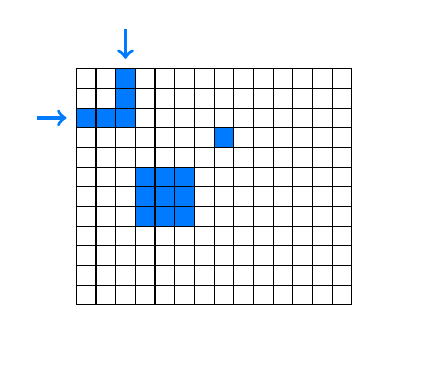
\begin{tikzpicture}
                \node at (-0.5,0){};
                \node at (4,-3.5){};
                \draw[fill = blued] (0.5,0) rectangle++(0.25,-0.75) rectangle++(-0.75,0.25);
                \draw[fill = blued] (0.75,-1.25) rectangle++(0.75,-0.75); 
                \draw[fill = blued] (1.75,-0.75) rectangle++(0.25,-0.25);
                \draw[very thick, blued, ->] (0.625,0.5) to ++(0,-0.375);
                \draw[very thick, blued, ->] (-0.5,-0.625) to ++(0.375,0);
                \foreach \x in {0,...,13}
                    \foreach \y in {0,...,11} 
                        {\draw ({\x*0.25},{\y*-0.25}) rectangle++(0.25,-0.25);}
            \end{tikzpicture}
            \subcaption{\texttt{free} vor der Platzierung}
            \label{fig:wg_placement_sub1}
        \end{subfigure}\hspace*{2bp}
        \begin{subfigure}[b]{0.4\textwidth}
            \centering
                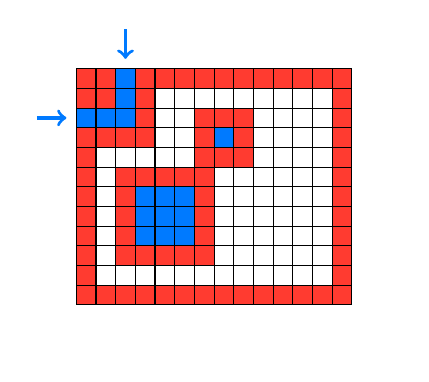
\begin{tikzpicture}
                    \node at (-0.5,0){};
                    \node at (4,-3.5){};
                    \draw[fill = redd] (0,0) rectangle++(3.5,-3);
                    \draw[fill = white] (0.25,-0.25) rectangle++(3,-2.5);
                    \draw[fill = redd] (0.25,-0.25) rectangle++(0.75,-0.75);
                    \draw[fill = redd] (0.5,-1.25) rectangle++(1.25,-1.25);
                    \draw[fill = blued] (0.5,0) rectangle++(0.25,-0.75) rectangle++(-0.75,0.25);
                    \draw[fill = blued] (0.75,-1.5) rectangle++(0.75,-0.75); 
                    \draw[fill = redd] (1.5,-0.5) rectangle++(0.75,-0.75);
                    \draw[fill = blued] (1.75,-0.75) rectangle++(0.25,-0.25);
                    \draw[very thick, blued, ->] (0.625,0.5) to ++(0,-0.375);
                    \draw[very thick, blued, ->] (-0.5,-0.625) to ++(0.375,0);
                    \foreach \x in {0,...,13}
                        \foreach \y in {0,...,11} 
                            {\draw ({\x*0.25},{\y*-0.25}) rectangle++(0.25,-0.25);}
                \end{tikzpicture}
                \subcaption{Anwendung der Filter}
                \label{fig:wg_placement_sub2}
            \end{subfigure}
        \vfill\hfill
        \begin{subfigure}[b]{0.4\textwidth}
            \centering
                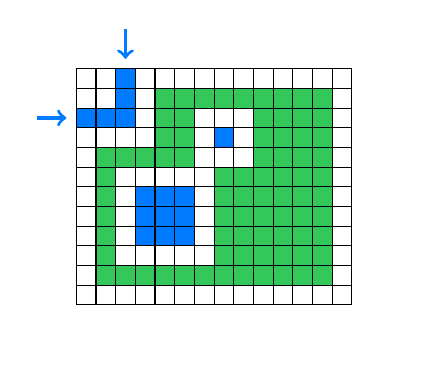
\begin{tikzpicture}
                    \node at (-0.5,0){};
                    \node at (4,-3.5){};
                    \draw[fill = white] (0,0) rectangle++(3.5,-3);
                    \draw[fill = greend] (0.25,-0.25) rectangle++(3,-2.5);
                    \draw[fill = white] (0.25,-0.25) rectangle++(0.75,-0.75);
                    \draw[fill = white] (0.5,-1.25) rectangle++(1.25,-1.25);
                    \draw[fill = blued] (0.5,0) rectangle++(0.25,-0.75) rectangle++(-0.75,0.25);
                    \draw[fill = blued] (0.75,-1.5) rectangle++(0.75,-0.75); 
                    \draw[fill = white] (1.5,-0.5) rectangle++(0.75,-0.75);
                    \draw[fill = blued] (1.75,-0.75) rectangle++(0.25,-0.25);
                    \draw[very thick, blued, ->] (0.625,0.5) to ++(0,-0.375);
                    \draw[very thick, blued, ->] (-0.5,-0.625) to ++(0.375,0);
                    \foreach \x in {0,...,13}
                        \foreach \y in {0,...,11} 
                            {\draw ({\x*0.25},{\y*-0.25}) rectangle++(0.25,-0.25);}
                \end{tikzpicture}
                \subcaption{Mögliche Positionen}
                \label{fig:wg_placement_sub3}
            \end{subfigure}\hspace*{2bp}
            \begin{subfigure}[b]{0.4\textwidth}
                \centering
                    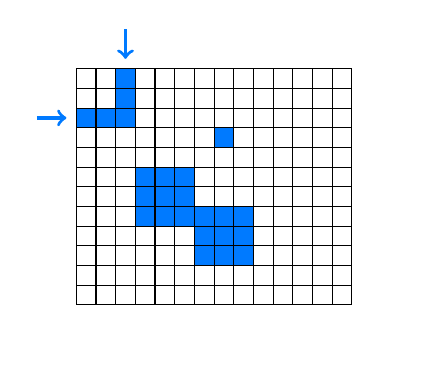
\begin{tikzpicture}
                        \node at (-0.5,0){};
                        \node at (4,-3.5){};
                        \draw[fill = blued] (0.5,0) rectangle++(0.25,-0.75) rectangle++(-0.75,0.25);
                        \draw[fill = blued] (0.75,-1.25) rectangle++(0.75,-0.75);
                        \draw[fill = blued] (1.5,-1.75) rectangle++(0.75,-0.75); 
                        \draw[fill = blued] (1.75,-0.75) rectangle++(0.25,-0.25);
                        \draw[very thick, blued, ->] (0.625,0.5) to ++(0,-0.375);
                        \draw[very thick, blued, ->] (-0.5,-0.625) to ++(0.375,0);
                        \foreach \x in {0,...,13}
                            \foreach \y in {0,...,11} 
                                {\draw ({\x*0.25},{\y*-0.25}) rectangle++(0.25,-0.25);}
                    \end{tikzpicture}
                    \subcaption{\texttt{free} nach der Platzierung}
                    \label{fig:wg_placement_sub4}
                \end{subfigure}\hfill
        \caption[Platzierung eines Objektes]{Beispiel: Platzierung eines Objektes der Größe $3\times 3$ in einem Level, in dem sich oben links ein freier Pfad und zwei bereits platzierte Objekte befinden. Blau markierte Quadrate entsprechen einem \texttt{false}-Eintrag im \texttt{free} Array.}
        \label{fig:wg_placement}
    \end{figure}

\subsection{Generierung des Terrains}
Die Spielwelt ist ein Unity Terrain quadratischer Größe. Dem Terrain ist eine Heightmap zugeordnet, über die die Höhe eines Punktes auf dem Terrain gesetzt werden kann. Die Heightmap hat den Wertebereich $[0,1]$ und wird um einen festgelegten Wert skaliert. Abhängig von der Ausgabe des zuvor beschriebenen Space Partitioning Algorithmus werden Masken in der Größe des Terrains generiert. Die Masken wählen Bereiche in der Spielwelt aus, die mit verschiedenen Operationen modifiziert werden, um eine Abgrenzung zwischen Levels, Korridoren und Zwischenräumen zu erhalten.
\subsubsection{Masken}\label{sec:terrainmask}
Die Spielwelt besteht aus Levels, Korridoren und Zwischenräumen. Das Spiel findet in den Levels und Korridoren statt. Die Zwischenräume werden mit Bergen gefüllt, wobei nicht vorgesehen ist, dass der Spieler die Zwischenräume betritt. Die Oberfläche des Terrains muss entsprechend modifiziert werden. Dazu werden Masken generiert, die Levels, Korridore und Zwischenräume auf dem Terrain maskieren. Die Masken sind zweidimensionale \texttt{bool} Arrays, die die gleiche Größe wie das Terrain haben. Damit ist jedem ganzzahligen Punkt auf der Oberfläche des Terrains ein Wert vom Typ \texttt{bool} zugeordnet. Grundlegend werden drei Masken generiert. \begin{itemize}
    \item Die Maske \texttt{levels} wird aus der unmittelbaren Ausgabe des Space Partitioning Algoritmus generiert und maskiert alle Positionen auf dem Terrain, die in einem Level liegen.
    \item Die Maske \texttt{corridors} maskiert alle Positionen durch die ein Korridor führt.
    \item Die Maske \texttt{intermediate} maskiert die Zwischenräume und wird für die Generierung von Bergen genutzt. Die Maske wird durch Invertierung der Addition der Masken \texttt{levels} und \texttt{corridors} gebildet.
\end{itemize}
Weitere Masken können durch Invertierung, Addition, Subtraktion und weitere Operationen erstellt werden. In Abbildung \ref{fig:wgmasks} sind die Masken \texttt{levels}, \texttt{corridors} und \texttt{intermediate} einer Spielwelt der Größe $512\times 512$ dargestellt. Dabei sind Positionen, an denen die Maske den Wert \texttt{true} enthält schwarz markiert und nicht maskierte Positionen sind grau markiert.

\begin{figure}
    \centering
    \begin{subfigure}[b]{0.25\textwidth}
        \centering        
        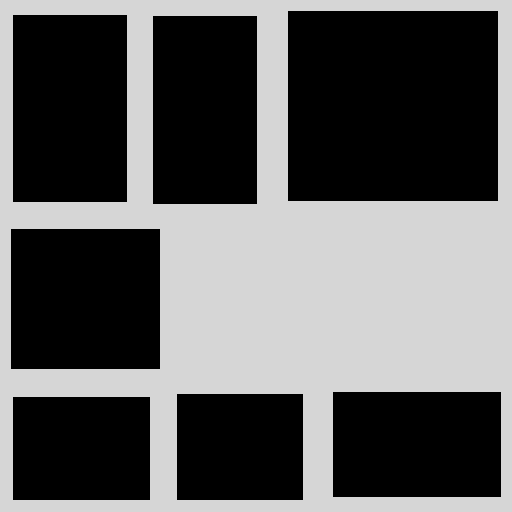
\includegraphics[width = \textwidth]{resources/img/wg/wgtmod_masks_levels.png}
        \caption{\texttt{levels}}
    \end{subfigure}
    \hspace{10bp}
    \begin{subfigure}[b]{0.25\textwidth}
        \centering
        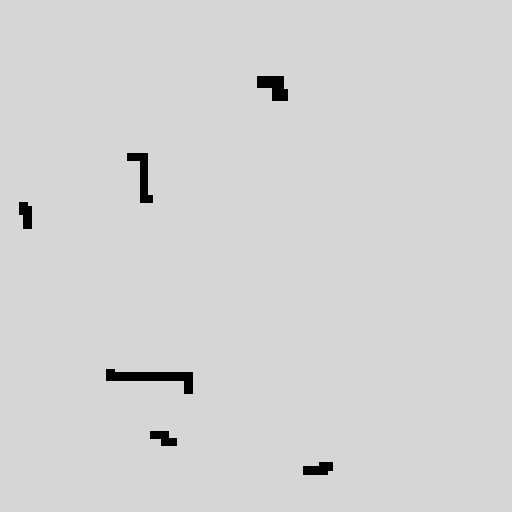
\includegraphics[width = \textwidth]{resources/img/wg/wgtmod_masks_corridors.png}
        \caption{\texttt{corridors}}
    \end{subfigure}\hspace{10bp}
    \begin{subfigure}[b]{0.25\textwidth}
        \centering        
        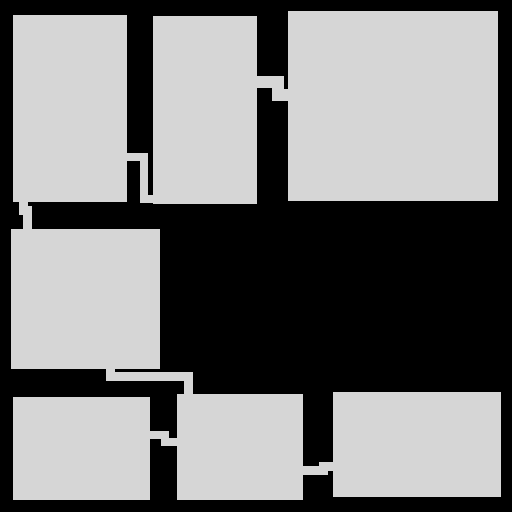
\includegraphics[width = \textwidth]{resources/img/wg/wgtmod_masks_intermediate.png}
        \caption{\texttt{intermediate}}
    \end{subfigure}\hfill
    \caption{Masken}
    \label{fig:wgmasks}
\end{figure}

\subsubsection{Heightmap Operationen}\label{sec:heightopt}
Zur Modifizierung der Heightmap stehen die Operationen \texttt{SetByMask}, \texttt{AverageFilter}, \texttt{PerlinNoise} und \texttt{Power} zur Verfügung. Die Operationen modifizieren die Höhen der Heightmap an den Positionen, die von einer als Eingabe geforderten Maske ausgewählt sind.
\begin{itemize}
    \item \texttt{SetByMask} wird mit einem Parameter vom Typ \texttt{float} aufgerufen. Die Operation ersetzt an maskierten Positionen die Höhe der Heightmap durch den gegebenen Parameter. Alle nicht maskierten Positionen bleiben erhalten, bzw. können durch einen optionalen Parameter vom Typ \texttt{float} auf einen Wert gesetzt werden.
    \item \texttt{AverageFilter} faltet die Heightmap mit einem Faltungsfilter der Größe $3\times 3$. Der Filter ist durch \begin{displaymath}
        F_{\text{Avg}}=\begin{bmatrix}
            \frac{1}{9}&\frac{1}{9}&\frac{1}{9}\\
            \frac{1}{9}&\frac{1}{9}&\frac{1}{9}\\
            \frac{1}{9}&\frac{1}{9}&\frac{1}{9}
        \end{bmatrix}
    \end{displaymath}
    gegeben und berechnet an jedem Punkt der Heightmap den Mittelwert in einem Radius von $1$.
    \item \texttt{PerlinNoise} addiert an maskierten Positionen den Wert einer Perlin-Noise Funktion auf die in der Heightmap gespeicherten Höhe. Dabei kann über Parameter die Skalierung des Perlin-Noise reguliert werden.
    \item \texttt{Power} erhält einen Parameter $z$ vom Typ \texttt{float}. Jeder maskierte Eintrag $v$ der Heightmap wird durch $v^z$ ersetzt.
\end{itemize}
Abbildung \ref{fig:wgtmodex} zeigt die Operationen am Beispiel eines Terrains der Größe $64\times 64$ mit einer Maske, die eine mittig liegende quadratische Fläche auswählt.

\begin{figure}
    \centering\hfill
    \begin{subfigure}[b]{0.4\textwidth}
        \centering        
        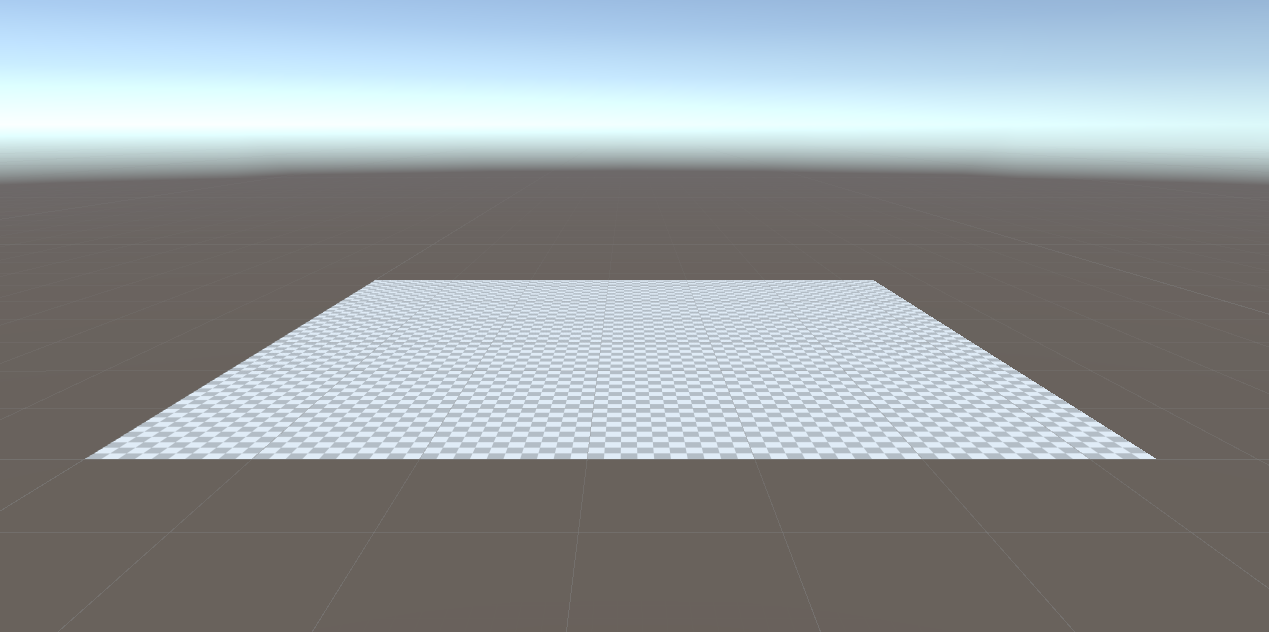
\includegraphics[width = \textwidth]{resources/img/wg/wgtmod_s.png}
        \caption{Terrain ohne Modifikation}
    \end{subfigure}
    \hspace{2bp}
    \begin{subfigure}[b]{0.4\textwidth}
        \centering
        
\includegraphics[width = 0.6\textwidth]{resources/img/wg/wgtmod_examplemask.png}
        \caption{Maske}
    \end{subfigure}\vfill\hfill
    \begin{subfigure}[b]{0.4\textwidth}
        \centering        
        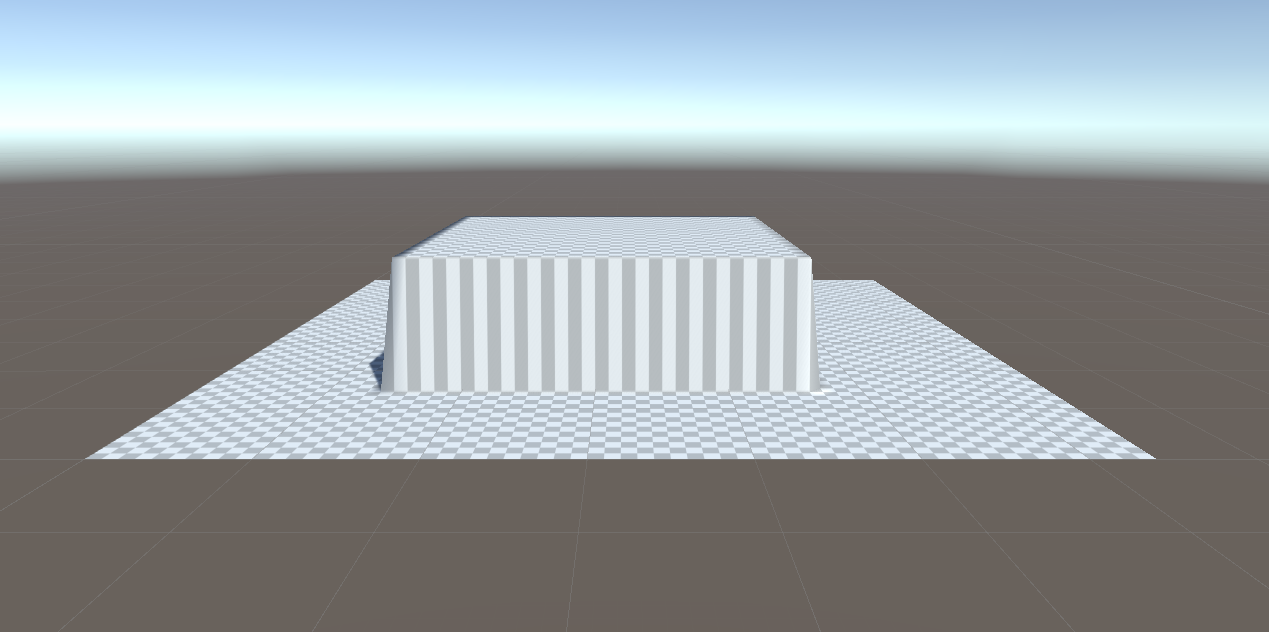
\includegraphics[width = \textwidth]{resources/img/wg/wgtmod_setbymask.png}
        \caption{\texttt{SetByMask}}
    \end{subfigure}
    \hspace{2bp}
    \begin{subfigure}[b]{0.4\textwidth}
        \centering
        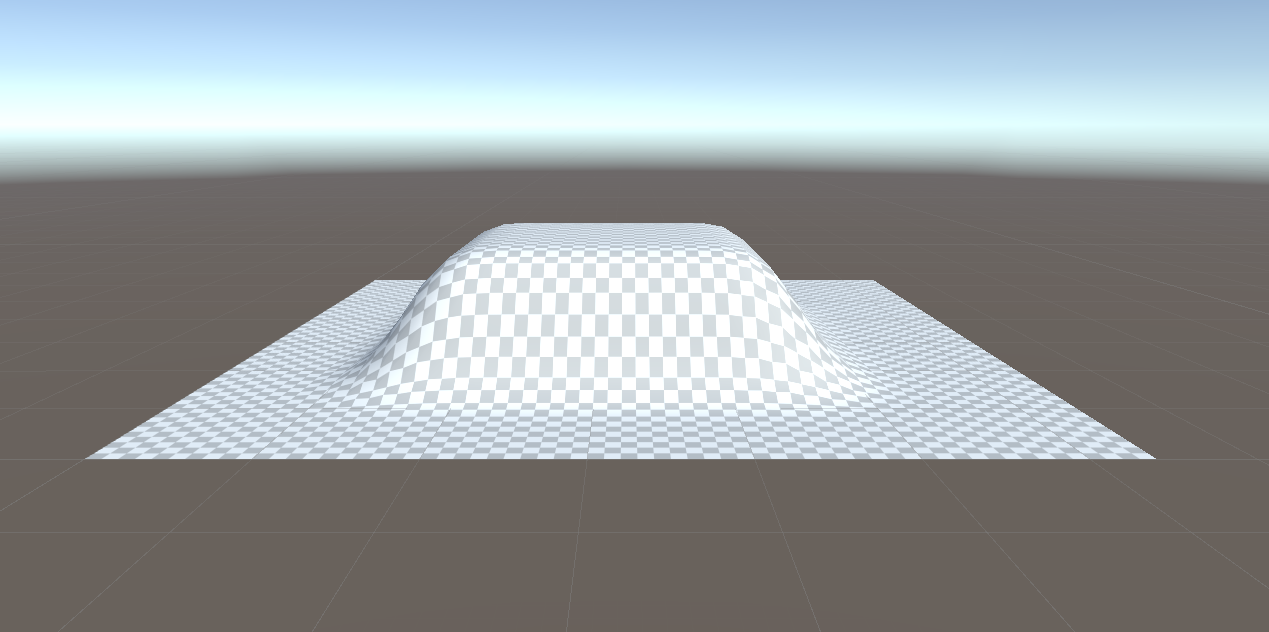
\includegraphics[width = \textwidth]{resources/img/wg/wgtmod_setbymask_avg.png}
        \caption{\texttt{SetByMask + AverageFilter}}
    \end{subfigure}\vfill\hfill
    \begin{subfigure}[b]{0.4\textwidth}
        \centering        
        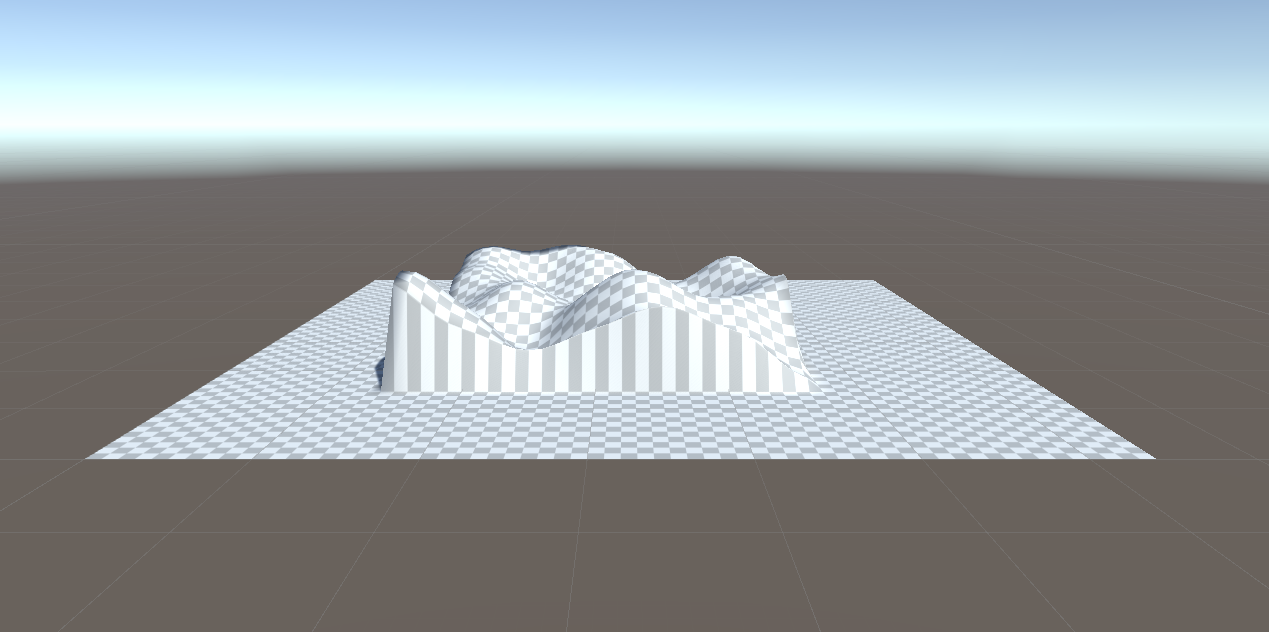
\includegraphics[width = \textwidth]{resources/img/wg/wgtmod_perlin.png}
        \caption{\texttt{PerlinNoise}}
    \end{subfigure}
    \hspace{2bp}
    \begin{subfigure}[b]{0.4\textwidth}
        \centering
        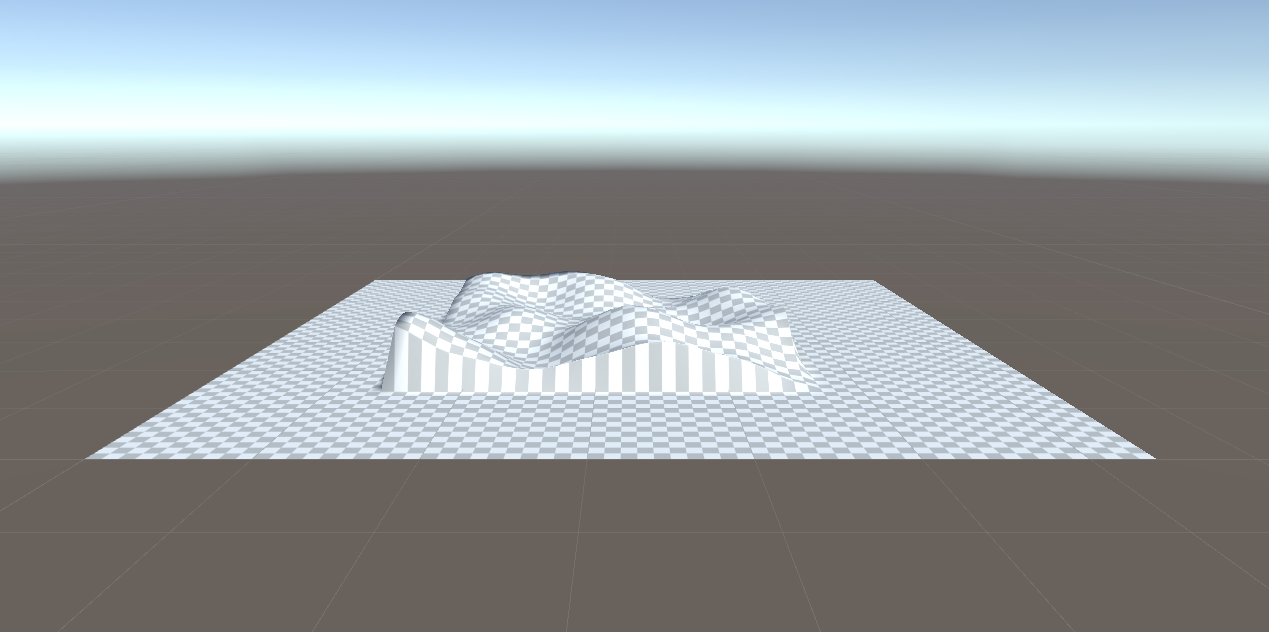
\includegraphics[width = \textwidth]{resources/img/wg/wgtmod_perlin_power.png}
        \caption{\texttt{PerlinNoise + Power(1.2)}}
    \end{subfigure}\hfill
    \caption[Operationen zur Modifikation der Heightmap des Terrains]{Operationen zur Modifikation der Heightmap des Terrains}
    \label{fig:wgtmodex}
\end{figure}
